
\documentclass[dvipdfmx,autodetect-engine]{jreport}
\usepackage[top=30truemm,bottom=30truemm,left=25truemm,right=25truemm]{geometry}
\usepackage[dvipdfmx]{graphicx}
\usepackage{float}
\usepackage{natbib}
\usepackage{subfig}
\usepackage[japanese]{minitoc}

\title{タイコグラフィによる回転体x線結像ミラーのキャラクタリゼーション}
\author{dieu.detruit }
\date{december 2020}

\renewcommand{\baselinestretch}{1.2}

\atbegindocument{
\dominitoc
}

\begin{document}

\begin{center}
\thispagestyle{empty}
{\large 令和2年度 卒業論文}\\
\begin{figure}[h]
    \centering
    
\includegraphics[scale=0.4]{images/utility/utlogo.jpg}
\end{figure}
\vspace*{2.5cm}
{\huge タイコグラフィ法による}\\
\vspace*{0.5cm}
{\HUGE 回転体X線結像ミラーの}\\
\vspace*{0.5cm}
{\huge キャラクタリゼーション}\\
\vspace*{1.5cm}
{\huge Characterization of Rotation X-ray Imaging Mirror}\\
\vspace*{0.5cm}
{\huge Using Ptychographical Method}\\
\vspace*{3.5cm}
{\large 指導教員 三村 秀和 准教授}\\
\vspace*{1.0cm}
{\large 東京大学 工学部 精密工学科}\\
{\large 03-190395}\\
\vspace*{1.0cm}
{\large 渡辺 貴史}
\end{center}

\newpage
\tableofcontents

% chapter1
\newpage
\chapter{序論}
\minitoc

\newpage
\section{研究の意義・背景}
通常、我々が天体を観測するとき、可視光を通してその形状や特徴を観察する。
一方で、天文学では熱や電磁波、放射線といった可視光以外の媒体を通じて様々な現象が明らかにされてきた。
中でも、電磁波の一種であるx線を観測することは、天文学において非常に有用である。
2018年に打ち上げられたfoxsi3では太陽コロナのx線写真を撮影することに成功し、その物理をより明らかにするに至った。
図\ref{fig:foxsi-fullsun-image}はその撮影像の1枚である。
太陽コロナを満たす高温のプラズマから放射される電磁波はX線の領域であり、これを撮影することは長年の課題であった。
X線は大気により吸収されやすいという特徴を持つため、宇宙に打ち上げられたロケットから観察する必要があるためである。
さらに、時間分解能と空間分解能の両方を十分に確保して撮影しなければならず、非常に難しい問題であった。
これを可能にした一つの要素として、Wolter型ミラーが挙げられる。

\begin{figure}[h!]
\centering
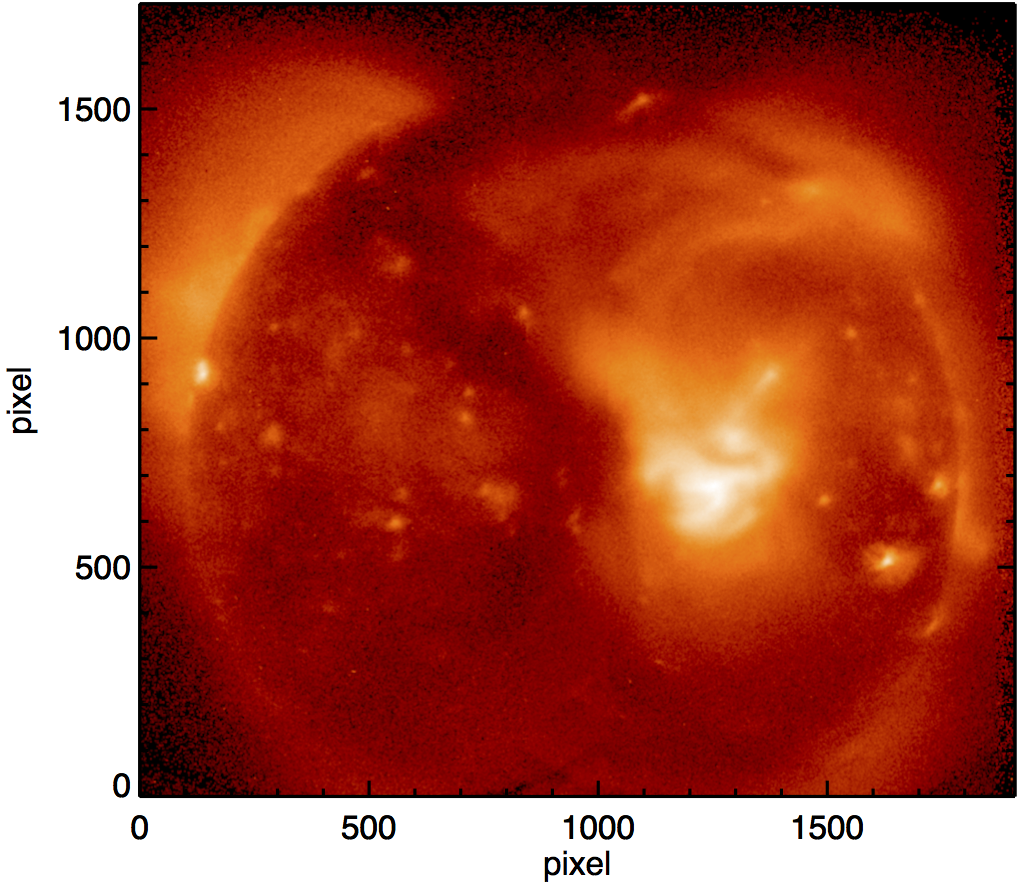
\includegraphics[scale=1.0]{images/foxsi/foxsi3-full-sun.png}
\caption{foxsi-3 phoenix full sun soft x-ray image}
\label{fig:foxsi-fullsun-image}
\end{figure}

\section{Wolterミラー}

光を一点に集光するための素子として、屈折を利用するレンズ、反射を利用したミラー、回折を利用したフレネルゾーンプレートなどが有名である。

WolterミラーにはI型、II型、III型の3種類が存在し(図hoge)、それぞれに長所と短所が存在する。
I型は内面において反射
II型は焦点距離が短くできる
III型は実用化されていない

\section{本研究で測定対象となるWolterミラーの設計}
本研究において測定対象となるのは、FOXSI-4での利用が検討されている天体望遠鏡用のWolterミラーであり、放物面、双曲面の順に反射するI型に分類される。
現在、回転体ミラーの加工では凸形状のマンドレルを高精度に加工し、そこに金属材料を転写するという方式が非常に有利であり、反射面がいずれも内側になるWolter I型が採用されている。
以下では、開発対象となっているWolter I型のミラーの設計パラメータを図\ref{fig:wolter_params}に対応して表\ref{tb:wolter_params}に示す。

\begin{figure}[h!]
\centering
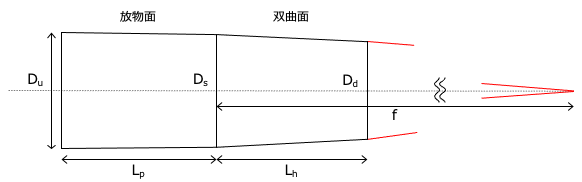
\includegraphics[scale=0.55]{images/mirror_experiment/mirror_params.png}
\caption{Wolterミラーの設計変数}
\label{fig:wolter_params}
\end{figure}

\begin{center}
  \begin{tabular}{|c|c|l|} \hline
    変数 & 値 & 説明 \\ \hline
    $d_u$ & 60.801 mm & 上流端開口直径 \\
    $d_s$ & 60.000 mm & 接合部直径 \\
    $d_d$ & 57.689 mm & 下流端開口直径 \\
    $l_p$ & 102.501 mm & 放物面部長さ \\
    $l_h$ & 97.499 mm & 双曲面部長さ \\
    $ml$ & 200.000 mm & ミラー全長 \\
    $f$ & 2000.000 mm & 焦点距離 \\ \hline
  \end{tabular}
  \label{tb:wolter_params}
  \caption{Wolterミラー各設計変数の値}
\end{center}

これらを図\ref{fig:wolter_profile}のように放物面部および双曲面部の設計半径として表すと、下式(パラメータは図\ref{tb:wolter_profile_constants})のようになる。

\begin{equation}
    r_p(z) = \sqrt{ -4p(z - p - f2) } \\
\end{equation}

\begin{equation}
    r_h(z) = b \sqrt{ \frac{(z - (f1 + f2) / 2)^2}{a^2} - 1.0 }
\end{equation}

\begin{figure}[h!]
\centering
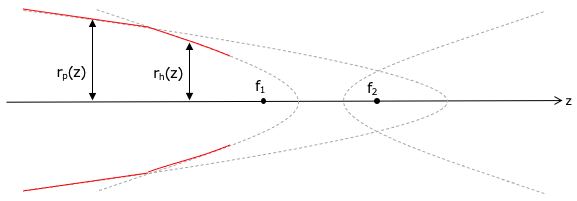
\includegraphics[scale=0.55]{images/mirror_experiment/mirror_profile.png}
\caption{Wolterミラーの設計半径}
\label{fig:wolter_profile}
\end{figure}

\begin{table}[htb]
    \begin{center}
      \begin{tabular}{|c|c|l|} \hline
        定数 & 値 & 説明 \\ \hline
        $p$ & 0.0562 mm & 下流端開口直径 \\
        $a$ & 1000.056 mm & 放物面部長さ \\
        $b$ & 10.606 mm & 双曲面部長さ \\ 
        $f1$ & 任意 & 焦点座標 \\
        $f2$ & $f1 + \sqrt{ a^2 + b^2 }$  & 共焦点座標 (双曲線のもう一方の焦点) \\\hline
      \end{tabular}
      \label{tb:wolter_profile_constants}
      \caption{Wolterミラーの設計半径における定数}
    \end{center}
\end{table}

\section{従来的な直接計測法}

\newpage
% chapter2
\chapter{Wolterミラーの誤差応答シミュレーション}
\minitoc

\newpage
\section{諸言}
Wolterミラーを光学系に組み込んで利用する際、大きく分けて2つの誤差によってその理想の集光・結像が損なわれる。
ひとつは設計曲面と実際に加工されたミラー表面の形状の誤差、もうひとつはミラー設置時の位置・姿勢の誤差である。

これらを与えたとき集光点の様子がどのようになるか、また集光点の変化として許容できる誤差の範囲はどれほどなのかを見積もることは、Wolterミラー評価の重要な軸となる。
6章では、加工されたミラーに対して測定実験を行い、本章で計算した許容誤差との比較・検討を行う。

\section{誤差の評価と許容される誤差}
結像または集光を行う光学系の是非が、集光面での波面が理想からどれだけ離れているかということで評価されるということを先に述べた。
いま、理想の集光波面との差異を定量的に評価するためには、具体的な評価軸が必要である。
そこで主に用いられるのが、Strehl比、HPD、FWHMの3つの特徴量である。

\subsection{Strehl比}
主に集光光学系の文脈において、理想の集光状態を「回折限界集光」と呼ぶ。
回折限界集光の状態にあるかどうかを判別する1つの指標として用いられるのが、Strehl比である。
Strehl比とは、実際の集光波面における最大値と回折限界時の集光波面における最大値の比として定義される。
つまり、振幅を$i(\mathbf{r})$として

\[
r_{\mathrm{Strehl}} = \frac{ \max{\sqrt{i(\mathbf{r})} } }{ \max{ \sqrt{i_{\mathrm{ideal}}( \mathbf{r} )} } }
\]

と定まる。
図\ref{fig:strehl_explanation}にその模式的なグラフを示す。
Strehl比を評価する基準として、Marechal基準である\citep{bornwolf:1999:book}が知られている。
Marechal基準では、Strehl比が0.8以上であるときその系は回折限界集光をしている、とする。
この0.8という値には体系的な根拠はなく、解析・実験における経験的な指標として扱われている。
本論文では、この慣例を踏襲し、0.8を閾値としてstrehl比を評価する。

\begin{figure}[h!]
\centering
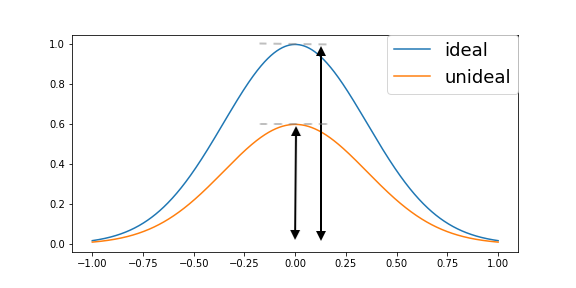
\includegraphics[scale=0.6]{images/error_simulation/explanation/strehl.png}
\caption{strehl比計算の模式図}
\label{fig:strehl_explanation}
\end{figure}

\subsection{hpd(half power diameter)}
strehl比による比較検討では「回折限界集光をしているか」に主眼を置いているが、天文用Wolterミラーのように達成すべき角度分解能が決まっている場合では、直接その分解能要求を満たしているかどうかを判定するのが実用的である。
分解能を決定するのは、焦点面におけるビームの集光サイズであり、これは大きく2つの定義によって議論される。
その一つが、Half Power Diameter(HPD)である。HPDの定義は「焦点面上の全強度の50\%の強度を含む円の直径」である。つまり、
\[
    \sum_{d\leq d_{\mathrm{hpd}}} \sqrt{ i(\mathbf{r}) } = \frac{1}{2} \sum \sqrt{ i(\mathbf{r}) }
\]
を満たすような直径$d_{\mathrm{hpd}}$として定義される。
図\ref{fig:hpd_explanation}にその例を示す。
この赤円の内側の強度総和値は、全体の強度総和値の半分になっている。

\begin{figure}[h!]
\centering
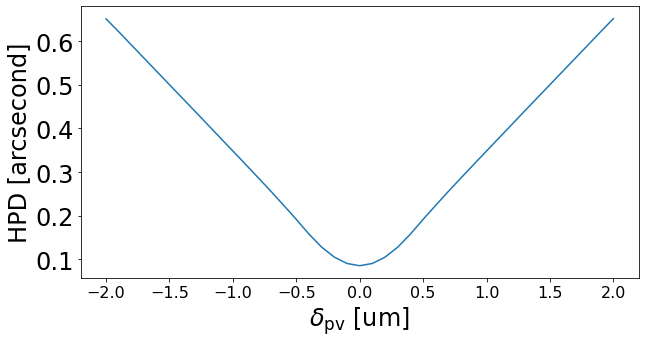
\includegraphics[scale=0.6]{images/error_simulation/explanation/hpd.png}
\caption{hpdの例}
\label{fig:hpd_explanation}
\end{figure}

\subsection{fwhm(full width half maximum)}
HPDに並んでビーム集光サイズの評価として用いられるのが、FWHM(Full Width Half Maximum)である。
こちらは焦点面を集光点を通る直線によって切断したプロファイルに対して、「焦点面における最大値の半分の値を取る2点の距離」と定められる。
図\ref{fig:fwhm_explanation_profile}は1つのプロファイルに対するFWHMの例である。
切断する直線には任意性があるため、通常は図\ref{fig:fwhm_explanation}のように水平方向と鉛直方向の切断しこれを評価する。

\begin{figure}[h]
\centering
\includegraphics[scale=0.6]{images/error_simulation/explanation/fwhm.png}
\caption{fwhmの例}
\label{fig:fwhm_explanation_profile}
\end{figure}

\begin{figure}[h!]
\centering

\subfloat[horizontal]{
    \includegraphics[scale=0.6]{images/error_simulation/explanation/fwhm_horizontal.png}
    \label{fig:fwhm_explanation_horizontal}
}
\subfloat[vertical]{
    \centering
    \includegraphics[scale=0.6]{images/error_simulation/explanation/fwhm_vertical.png}
    \label{fig:fwhm_explanation_vertical}
}
\caption[]{切断の例 水平:\subref{fig:fwhm_explanation_horizontal}, 鉛直:\subref{fig:fwhm_explanation_vertical}}
\label{fig:fwhm_explanation}
\end{figure}

\section{Wolterミラーにおける光学波動場の伝播}
本節では、本研究で測定対象とするWolterミラーの系において適用するべき波動場伝播の近似公式について説明する。
光学波動場の伝播に関しての詳細は付録において解説する。

\section{シミュレーションの方法}
この節では、シミュレーションの方法について述べる。

\section{計算条件}
6章で実際に利用する測定対象のミラーについて、誤差応答のシミュレーションを行う。


\section{直径誤差}

\section{扁平誤差}

\section{周方向形状誤差}

\section{長手方向形状誤差}

\section{設置角度誤差}

\section{設置位置誤差}

\newpage
% chapter3
\chapter{Wolterミラー評価実験の手法に関する検討}
\minitoc

\newpage
\section{位相回復法の概要}
2章でも述べた通り、波面計測は波動光学に基づいており、x線の伝播は複素波動場として与えられる。
一方で、CCDカメラなどの撮像素子で得られるのはその振幅の2乗、つまりエネルギーの情報のみである。
つまり、求めたい複素波動場に対して、カメラによる撮影では位相の情報を計測することができない。
一般にこれは位相回復問題と呼ばれ、様々な解決方法が提案されている。

いま、位相回復問題とは計測対象の画素数を縦横とも$n$として、$n \times n$の計測値を元に$n \times n$の未知数を求めることと定式化できる(図\ref{fig:phase_retrieval_problem})。
位相回復法では、どの方法においても共通の方針を取る。
未知数を求めるためには、それらを含む方程式を十分な数立てることが必要だが、一般に求める光学波動場において強度と位相の間に拘束関係はない。
そこで、焦点面に加えてもう1つ平面を定義し、その平面と焦点面の間の光学波動場の伝播を関係式として与えることで、未知数は増えるもののそれらを含む方程式を得ることができる。
これを図\ref{fig:phase_retrieval_policy}に示す。
波動場の伝播はkirhihoff-helmholtz方程式の解として表され、距離や開口サイズに応じて近似公式が多く知られている。中でも、十分遠方においてフーリエ変換の関係で表されることが知られている。これについては、appendixにおいて詳説する。
波動場の伝播は$n \times n$の離散領域に対して$n \times n$本の数式で表される。
これだけでは未知数が$3n \times \n$個に対して方程式が$n \times n$本と少なく、未知数を全て決定することができない。
そこで、未知数を減らす、もしくは関係式を増やすといった工夫を行うことで、解を決定するという方針を取る。

\begin{figure}[h!]
\centering
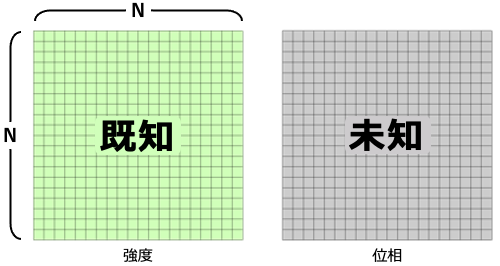
\includegraphics[scale=0.5]{images/phase_retrieval/phase_retrieval_problem.png}
\caption{位相回復問題}
\label{fig:phase_retrieval_problem}
\end{figure}

\begin{figure}[h!]
\centering
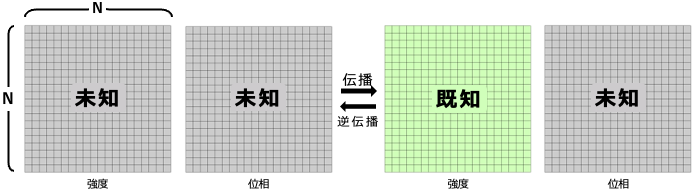
\includegraphics[scale=0.5]{images/phase_retrieval/phase_retrieval_policy.png}
\caption{位相回復法の方針}
\label{fig:phase_retrieval_policy}
\end{figure}

以下では、代表的な解法を紹介し、続いてそれらを用いた天文用Wolterミラーの波面計測に関するシミュレーションの結果を示す。

\section{疎条件の利用}
主にCDI(コヒーレント回折イメージング)の文脈において、波動場が到達しない領域を定数0として与えることで未知数をの総数を激減させるという方法が多く取られる。
CDIとは、図\ref{fig:cdi_schematic}に示すように、サンプルに集光ビームを照射し、その回折像を見ることでそのサンプルの内部構造を解析する方法である。
位相回復法によってディテクターでの位相およびサンプル面における位相・強度を求めることで、サンプル各点における透過率を求めることが目標となる。
このような系においては、カメラの画素をより細かく取ることにより、対応するサンプル面での領域がサンプルより大きく広がるため、この領域には波面が存在しないという仮定を用いて回復計算を行うことができる。
本研究で対象とするWolterミラーについても、回復の対象である輪帯状でかつ細い波面は、下流端開口面全体に対して面積が非常に小さく、同様の方法が有効である。
CDIで広く使われているアルゴリズムの1つが、HIO(Hybrid Iterative Engine)であり、この系にも適用することが可能である。以下にその概要を示す。

\section{タイコグラフィ法}
前節で述べた方法について、用いるオブジェクトには大きく分けて2種類ある。1つは透過関数として表現される


\section{ディテクター走査による冗長性}

\section{下流端開口走査による冗長性}

\subsection{対称性}

\newpage
% chapter4
\chapter{レンズによる提案手法の検討}
\minitoc

\newpage
\section{実験の構成および設計パラメータ}
実験装置の概要を以下に示す。
平行光に対して輪帯状の開口を入れることで、擬似的に輪帯開口の集光光学系を再現する。
輪帯開口の設計

レンズによる提案手法の検証に際して、本来の測定対象であるWolterミラーと同様の系を構成するべきであるが、入手性の問題からここではNAがほぼ等しいレンズを用いて実験を行う。
用いたレンズのパラメータは表\ref{tb:focusing_lens_params}に示す通りである。

\begin{table}
\begin{center}
  \begin{tabular}{|c|c|} \hline
    パラメータ & 値 \\ \hline
    直径 & 30.0 mm  \\
    焦点距離 & 1000.000 mm \\
    設計波長 & 500くらいnm \\ \hline
  \end{tabular}
  \label{tb:focusing_lens_params}
  \caption{レンズの設計パラメータ}
\end{center}
\end{table}

これに合わせて、輪帯開口およびピンホールを図\ref{fig:lens_pinhole_ring_aperture}の用に設計した。
輪帯幅を変えて実験を行うため、図\ref{fig:lens_ring_aperture}における$A$を表\ref{tb:lens_ring_aperture_inner_diameter}のように3通り用意した。

\begin{figure}[h!]
\centering

\subfloat[ピンホール]{
    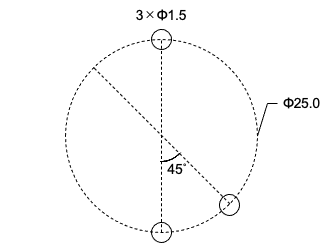
\includegraphics[scale=0.5]{images/lens_experiment/pinhole_arrangement.png}
    \label{fig:lens_pinhole_arrangement}
}
\subfloat[輪帯アパーチャ]{
    \centering
    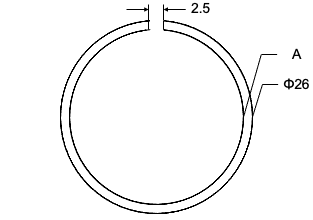
\includegraphics[scale=0.5]{images/lens_experiment/ring_aperture.png}
    \label{fig:lens_ring_aperture}
}
\caption[]{設計図面}
\label{fig:lens_pinhole_ring_aperture}
\end{figure}

\begin{center}
  \begin{tabular}{|c|c|l|} \hline
    番号 & A \\ \hline
    1 & 25 mm  \\
    2 & 25.5 mm  \\
    3 & 25.75 mm \\ \hline
 \hline
  \end{tabular}
  \label{tb:lens_ring_aperture_inner_diameter}
  \caption{輪帯アパーチャ内円の直径}
\end{center}

\newpage
% chapter5
\chapter{ミラー計測実験}
\minitoc

\newpage
\section{実験の構成}
実験装置の概要を以下に示す。図\ref{fig:mirror_experiment_asm_cad_side}が横から見たcad図、図\ref{fig:mirror_experiment_asm_cad_isometric}が俯瞰して見た図である。

\begin{figure}[h!]
\centering
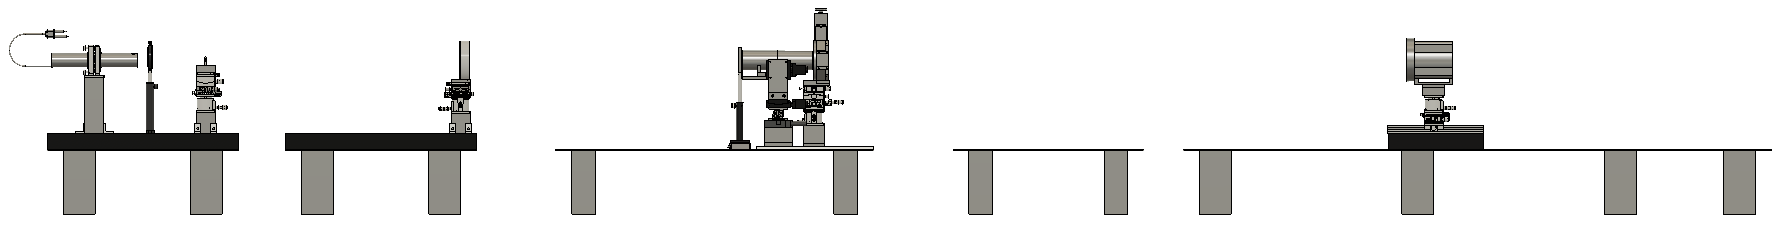
\includegraphics[scale=0.25]{images/mirror_experiment/setup/asm_total_side.png}
\caption{ミラー測定実験系 側面図}
\label{fig:mirror_experiment_asm_cad_side}
\end{figure}

\begin{figure}[h!]
\centering
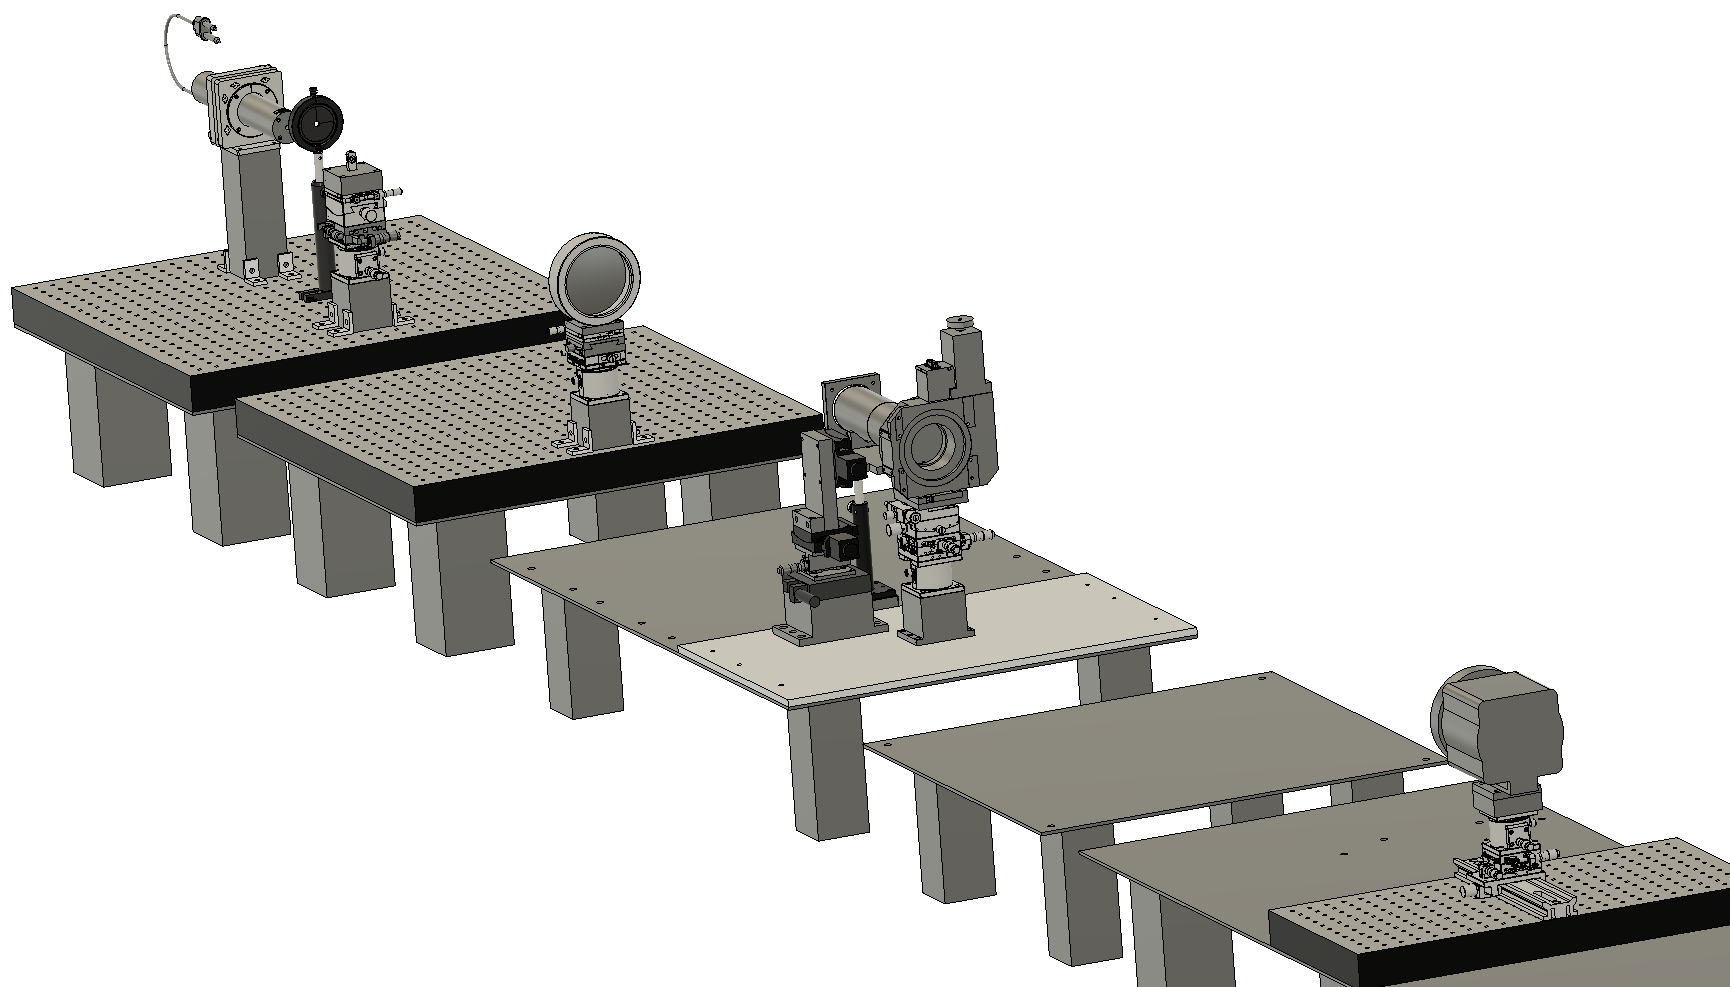
\includegraphics[scale=0.25]{images/mirror_experiment/setup/asm_total_isometric.png}
\caption{ミラー測定実験系 俯瞰図}
\label{fig:mirror_experiment_asm_cad_isometric}
\end{figure}

\newpage
% chapter6
\chapter{結論}
\minitoc

\newpage
``i always thought something was fundamentally wrong with the universe'' \citep{adams1995hitchhiker}


\newpage
\chapter{付録}
\minitoc

\section{光学波動場の伝播}
\subsection{Kirhihoff-Helmholtz方程式}

\subsection{Rayleigh-Sommerfeldの回折積分公式}

\subsection{Rayleigh-Sommerfeldの高速計算}

\subsection{Fresnel回折積分}

\subsection{Fraunhofer回折積分}

\subsection{角スペクトル法}

\newpage
\bibliographystyle{plain}
\bibliography{references}

\chapter*{謝辞}
本当にありがとうございました。

\end{document}

